% "storage along flow path": resolved (a storage at every position) or averaged (one storage)
\documentclass[tikz, border=4pt]{standalone}
% Shared preamble of the PyTES model diagrams: packages, colours and styles.
% Each diagram is a standalone document that inputs this file; build them with build.py.
\usepackage{amsmath}
\usepackage{bm}
\usetikzlibrary{arrows.meta, calc, decorations.pathreplacing, patterns, positioning}

% The PyTES Thermal colour cycle (pytes.plotting.THERMAL) and tints of it
\definecolor{pytesorange}{HTML}{E8590C}
\definecolor{pytesblue}{HTML}{1F4E9C}
\definecolor{pytesteal}{HTML}{14A08A}
\definecolor{pytesamber}{HTML}{F0A930}
\definecolor{pytesplum}{HTML}{A23B72}
\definecolor{pytessky}{HTML}{88C7F0}
\definecolor{pytesink}{HTML}{36312E}

% Materials: the heat transfer fluid, the PCM, the metal (fins and tubes)
\colorlet{fluidfill}{pytessky!75}
\colorlet{pcmfill}{pytesamber!55}
\colorlet{liquidfill}{pytesorange!60}
\colorlet{metalfill}{pytesink!45}
\colorlet{compositefill}{pcmfill!85!metalfill}

\tikzset{
  >={Stealth[length=2.2mm]},
  every picture/.style={line join=round, line cap=round, font=\small},
  outline/.style={draw=pytesink, line width=0.6pt},
  fluid/.style={outline, fill=fluidfill},
  pcm/.style={outline, fill=pcmfill},
  liquid/.style={outline, fill=liquidfill},
  metal/.style={outline, fill=metalfill},
  composite/.style={outline, fill=compositefill},
  flow/.style={->, draw=pytesblue, line width=1.2pt},
  heat/.style={->, draw=pytesorange, line width=1.1pt},
  axis/.style={->, draw=pytesink, line width=0.7pt},
  dimension/.style={<->, >={Stealth[length=1.6mm]}, draw=pytesink, line width=0.5pt},
  guide/.style={draw=pytesink!60, line width=0.4pt, dashed},
  symmetry/.style={draw=pytesink, line width=0.5pt, dash dot},
  label/.style={text=pytesink, font=\small},
  note/.style={text=pytesink, font=\footnotesize, align=center},
}

\begin{document}
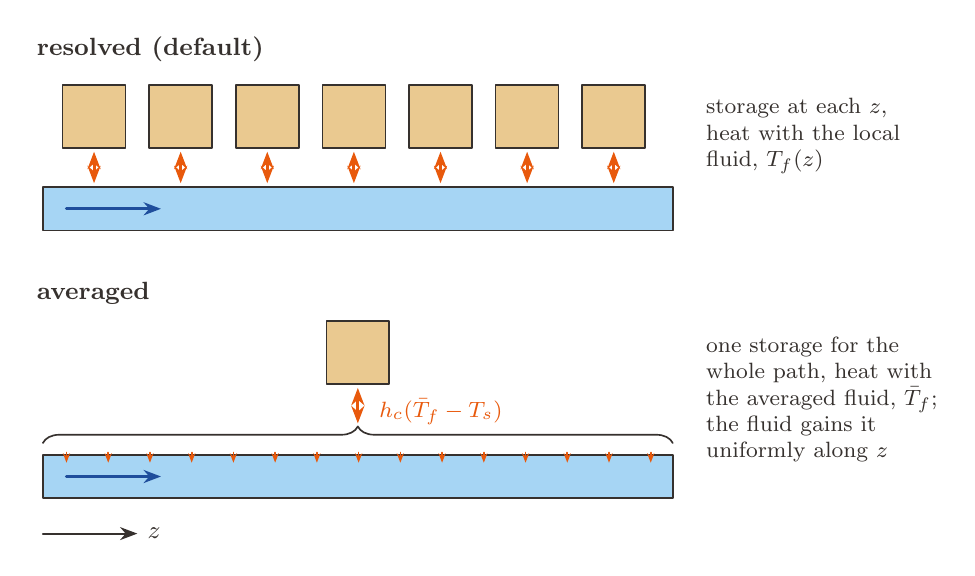
\begin{tikzpicture}
  \def\L{8.0}
  % Resolved: one storage cross-section at each position, exchanging with the local fluid
  \begin{scope}[shift={(0, 3.4)}]
    \node[label, anchor=west, font=\small\bfseries] at (-0.2, 2.3) {resolved (default)};
    \draw[fluid] (0, 0) rectangle (\L, 0.55);
    \draw[flow] (0.3, 0.275) -- (1.5, 0.275);
    \foreach \i in {0, ..., 6} {
      \draw[composite] ({0.25 + 1.1*\i}, 1.05) rectangle ({1.05 + 1.1*\i}, 1.85);
      \draw[heat, <->] ({0.65 + 1.1*\i}, 0.6) -- ({0.65 + 1.1*\i}, 1.0);
    }
    \node[note, anchor=west, align=left] at (\L + 0.3, 1.2)
      {storage at each $z$,\\heat with the local\\fluid, $T_f(z)$};
  \end{scope}
  % Averaged: one storage cross-section for the whole flow path
  \begin{scope}
    \node[label, anchor=west, font=\small\bfseries] at (-0.2, 2.6) {averaged};
    \draw[fluid] (0, 0) rectangle (\L, 0.55);
    \draw[flow] (0.3, 0.275) -- (1.5, 0.275);
    \draw[composite] (\L/2 - 0.4, 1.45) rectangle (\L/2 + 0.4, 2.25);
    \draw[decorate, decoration={brace, amplitude=6pt, mirror}, pytesink, line width=0.6pt]
      (\L, 0.7) -- (0, 0.7);
    \draw[heat, <->] (\L/2, 0.95) -- (\L/2, 1.4);
    \node[note, anchor=west, text=pytesorange] at (\L/2 + 0.15, 1.1)
      {$h_c (\bar T_f - T_s)$};
    \foreach \i in {0, ..., 14} {
      \draw[->, pytesorange, line width=0.6pt, >={Stealth[length=1.2mm]}]
        ({0.3 + 0.53*\i}, 0.58) -- ({0.3 + 0.53*\i}, 0.45);
    }
    \node[note, anchor=west, align=left] at (\L + 0.3, 1.25)
      {one storage for the\\whole path, heat with\\the averaged fluid, $\bar T_f$;\\the fluid gains it\\uniformly along $z$};
  \end{scope}
  \draw[axis] (0, -0.45) -- (1.2, -0.45) node[label, right] {$z$};
\end{tikzpicture}
\end{document}
